% !TeX spellcheck = de_DE
\chapter{Systemdesign}
\label{sec:design}
Die Softwareentwicklung beginnt mit einer Beschreibung der Bedürfnisse und ihrer Analyse. Je genauer und korrekter die Beschreibung der Softwareanforderungen und deren Analyse ist, desto einfacher ist es, alle nachfolgenden Schritte abzuschließen. Das Hauptproblem in dieser Phase ist der Unterschied in den Ansichten des Kunden (in dem Fall der vorliegenden Abschlussarbeit sind die Kunden die PSE-Labor Mitarbeiter) und des Entwicklers (die Autorin der Abschlussarbeit). Es wurde auch die Entscheidung getroffen, mit welchen Hardware ist die Aufgabestellung zu implementieren. Jedoch während der Entwicklung der Register-Client (der einer von drei Bestandsteilen der Software, an dem ein RFID-Leser angeschlossen werden muss), wurde schließlich ein RFID-Leser gewechselt. Der Fall ist im Kapitel \ref{sec:register_client:install_rfid} nachzulesen. Im Rahmen der Analyse und des Systemdesigns wurden die Struktur und Zusammenhänge der Elemente des zu entwickelnden Systems untersucht. Das Ergebnis dieser Untersuchung enthält genügend Informationen, um das System zu implementieren und ist unten in folgenden Kapitels detailliert beschrieben. 

\section{User Stories}
\label{sec:design:user_stories}
Zuerst wurden die User Stories erstellt, die eine diskutierte Darstellung der Absicht (Endbenutzer muss/will so etwas tun) zeigen können. Es ist mithilfe der User Stories zu klären, was die zu entwickelnde Datenbank leisten soll. Es wird auf die Frage konzentriert, welche Daten in der Datenbank gespeichert werden sollen. 
Der Text der User Story selbst sollte die Rolle / Aktionen des Benutzers im System, seine Bedürfnisse und den Gewinn erläutern, den der Benutzer nach dem Auftreten der Story erhält. Zum Beispiel: Wie \textit{<Benutzerrolle / Charakter>, ich <möchte etwas bekommen>, <für diesen und jenen Zweck>}. Während des Schreibens der User Story wurden zwei Gruppe von Stakeholders definiert: die Studierende (Beuth Studentinnen und Studenten) und der Admin (PSE-Labor Mitarbeitern). Es wurden die folgenden User Stories erstellt, die später während der Entwicklungsphase implementiert wurden:
\begin{itemize}
	\itemsep-1.2em 
	\item As a student, I want \textbf{to loan a board} so I can work at lab
	\item As a student, I want \textbf{to loan a board} so I can work at home
	\item As a student, I want \textbf{to list boards assigned to me} so that I am sure I to return
	\item As a student, I want \textbf{to return a board from lab work} so that I can loan again
	\item As a student, I want \textbf{to return a board from home work} so that I can loan again
	\item As a student, I want \textbf{to initiate session} so I can loan a board
	\item As a lab admin, I want \textbf{to mark a board} so it can be loaned for home or for lab
	\item As a lab admin, I want \textbf{to terminal session} with timeout so that students can use the loan station
	\item As a lab admin, I want \textbf{to block a student} so that they won't be able to loan a board
	\item As a lab admin, I want \textbf{to see all students} registered on the course so that I can manage their profiles
	\item As a lab admin, I want \textbf{to see all loaned boards} so that I can know their expected return date
	\item As a lab admin, I want \textbf{to register students} so that they are able to loan boards
	\item As a lab admin, I want \textbf{to register new boards} so that thay can be loaned
	\item As a lab admin, I want \textbf{to delete student's record} when semester ends so that they are not stored anymore in database
\end{itemize}


\section{Anforderungen}
\label{sec:design:req}
Während die meisten neuen Funktionen mithilfe der User Stories aus Anwendersicht definiert werden sollten, ist dies nicht immer machbar oder sogar hilfreich, wenn es zu Sicherheitsfunktionen oder Infrastrukturanforderungen kommt, die nicht kundenorientiert sind. Es gibt zwei Arten von Anforderungen: funktionale Anforderung und nichtfunktionale Anforderungen. Während der Analysephase wurden die beiden Arten von Anforderungen definiert. 

\subsection{Funktionale Anforderungen}
Eine funktionale Anforderung beschreibt, was ein Softwaresystem tun sollte. Es werden die folgenden funktionalen Anforderungen definiert:
\label{sec:design:req:func}
\begin{itemize}
	\itemsep-1.2em 
	\item The background color for all windows in the application will be white and have a hexadecimal RGB color value of 0x0000FF.
	\item The colors of design guidelines of Beuth Hochschule will be used.
	\item The software automatically validates whether a student is able to loan a board for a homework.
	\item The software automatically shows the information about boards that student already loaned.
	\item Student will see their name after they scanned their valid student card.
	\item Student will see board's number after they scanned a Raspberry Board.
	\item If student can not loan a board they will see an information message on a display.
	\item If a student can not loan a board the session should be terminated
	\item If an error during the loan proccess is occured the student will see datailed information so they can later talk with an admin about theis issue.
	\item Error states will be marked with red color on the page
	\item Succeeded states will be marked with a green color on the page
\end{itemize}

\subsection{Nichtfunktionale Anforderungen}
Nichtfunktionale Anforderungen bestimmen nicht die Funktionen, sondern die Eigenschaften des Systems: Leistung, Zuverlässigkeit, Verfügbarkeit, Skalierbarkeit und eine Reihe anderer Parameter, die das Systems einschränken und verbessern sollen. 
\label{sec:design:req:non-func}
\begin{itemize}
	\itemsep-1.2em 
	\item The Server has to be implemented using a modern Python web framework Django.
	\item The user Interfaces (frontend) shall be implemented as HTML pages with dynamic content inside based on Django Templates.
	\item The admin views must require authorization. A view decorated with this function will be executed normally only if the logged user has admin rights.
	\item The SQLite rational database will be used in order to store students, boards and loan records
	\item For terminating the session automatically after timeout the command line application (CLI) will be implemented using python and will be run on the server.
	\item Users must use for the initial login their student card. Moreover, every next login will be done with the same card. 
	\item Students never allowed to loan home board longer than 1 week (7 calendar days). Such attempt should be reported to the security administrator.
	\item Students never allowed to loan lab board longer than 120 minutes. An the end of the exercise admnistrator should be notified if the board was not returned.
	\item Loan process can not be started if a student was not properly registered on the course
	\item Every unsuccessful attempt by a user to loan/return an item shall be recorded on an audit trail.
	\item Only one active session is allowed for loan/return process. No multi-user mode is intended
	\item If the currect session is inactive longer longer than 180s the session will be terminated and should be restarted
	\item The actions made on RFID-Reader should be displayed on the screen with an acceptable delay for a humans (less then 5 seconds)
\end{itemize}

Während die User Story selbst die Verbindung zwischen der menschlichen Wahrnehmung und der technischen Umsetzung ist, können mithilfe der Anforderungen die Betriebsfunktionen und Einschränkungen des Systems beschrieben werden, die seine Funktionalität verbessern.

\section{Anwendungsfälle}
\label{sec:design:use_cases}
Anwendungsfalldiagramme beschreiben selbst kein Verhalten und keine Abläufe, sondern nur die Zusammenhänge zwischen einer Menge von Anwendungsfällen und den daran beteiligten Akteuren. Sie eignen sich daher besonders gut, um für Benutzer des Systems (Akteure) relevante funktionale Anforderungen an ein System zu analysieren\cite{website:21}. Während der Analyse der Systemanforderungen wurde es festgestellt, dass die Software aus vier zentralen Anwendungsfällen bestehen sollte. Diese sind: Die Ausleihe des Lab-Loan Boards, die Rückgabe des Lab-Loan Boards, die des Ausleihe des Home-Loan Boards, die Rückgabe des Home-Loan Boards. Jeder von diesen Anwendungsfälle kann erfolgreich oder mit dem Fehler beendet werden.

\subsection{Ausleihe des Lab-Loan Boards}
\label{sec:design:use_cases:lab_loan}
Ein Studierende soll während der Übung im PSE-Labor ein Lab-Loan Board für 120 Minuten ausleihen, um die Aufgaben der Lehrkraft zu erledigen. Die 120 Minuten entsprechen die 90 Minuten der Übung + zusätzlichen 15 Minuten vor und nach der Übung, um Board aus-/einzupacken, an-/auszuschalten und laufenden Arbeit am Ende der Übung zu speichern. 
Ein erfolgreichen Szenario besteht aus die folgenden Schritten: nachdem hat ein Studierende ein Lab-Loan Board aus dem Schrank genommen drückt er die Start-Taste am Bildschirm des Display-Client. Dann lässt er seine Studentenkarte am Register-Client über RFID-Leser abzulesen und danach sieht eine Begrüßung des Systems und seinen eigenen Name. Ein Studierende mithilfe des RFID-Lesers liest als nächsten der RFID-Tag des Lab-Loan Board ab, dessen Nummer wird nach dem Ablesen am Bildschirm des Display-Client unter dem Name der Studierende gezeigt. Dann muss die Taste "Loan Board" gedrückt werden. Nach der Bestätigung der Ausleihe drückt der Studierende eine Taste "Finish" und somit wird Anwendungsfall erfolgreich beendet. 

Jedoch sind auch Fehlerzustände für den Anwendungsfall vorgesehen. Falls der Studierende zum Kurs von Admin nicht registriert wurde, wird ein Ausleihvorgang nach dem Ablesen der Studentenkarte sofort mit der Fehlermeldung \textit{"Invalid student card"} im Fehlerzustand terminiert. Falls der Studierende hat schon einen Lab-Loan Board ausgeliehen und versucht jetzt einen weiteren an sich zuweisen, wird ein Ausleihvorgang sofort mit der Fehlermeldung \textit{"Same bord type"} im Fehlerzustand terminiert. Falls es auf einen Versuch käme, ein dritten Board auszuleihen, wird Fehlermeldung \textit{"Maximum boards reached"} angezeigt und sofort im Fehlerzustand terminiert. Falls ein nicht bekannte RFID-Tag am RFID-Leser anstatt der Lab-Boards wird abgelesen, kommt es zu einem Fehlerzustand \textit{"Status error"}, da ein RFID-Tag keinem Board mit irgendwelchen Zustand in System zugewiesen werden kann. 

\begin{figure}
	\centering
	\fbox{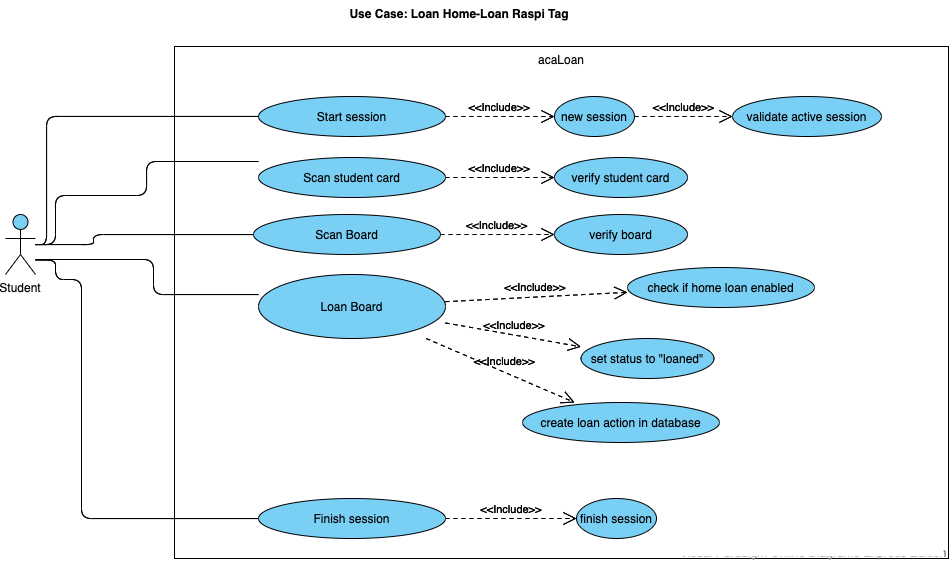
\includegraphics[width=1\textwidth]{gfx/home_loan.png}}
	\caption{UML Anwendungsfall: Ausleihe des Home-Loan Boards}
	\label{fig:use_home_loan}
\end{figure}

\subsection{Ausleihe des Home-Loan Boards}
\label{sec:design:use_cases:home_loan}
Der folgenden Anwendungsfall ist ähnlich zum vorherigen Anwendungsfall \textit{"Ausleihe des Lab-Loan Boards"} aus dem Kapitel \ref{sec:design:use_cases:lab_loan}. Der Home-Loan Board darf in diesem Fall für 7 Kalendertagen ausgeliehen werden. Es gibt jedoch einen wichtigen Unterschied zur Lab-Ausleihe: solange ein Student ein Teilnehmer des Moduls ist, kann es dem Studierende nicht verweigert werden, während der Übung des Lab-Loan Board für die Lösung der Aufgaben zu benutzen und auszuleihen. Jedoch für Home-Ausleihe gilt eine andere Regelung, wann es ihm die Home-Ausleihe-Absicht gesperrt werden kann. Falls das Gerät in einem sehr üblen Zustand der Verschmutzung oder Zerstörung ohne eine Besprechung mit dem Administrator zurückgegeben wurde, darf der Studierende ein Gerät nachsten Mal nicht ausleihen. Falls es auf einen Versuch käme, ein Home-Loan Board auszuleihen mit dem ungesetzten im Profil Flag $"home\_loan\_is\_enabled"$ , wird Fehlermeldung \textit{"Home loan disabled"} angezeigt und der die Sitzung sofort im Fehlerzustand terminiert.  Der oben geschrieben Anwendungsfall ist auf der Abbildung \ref{fig:use_home_loan} zu sehen.

\begin{figure}
	\centering
	\fbox{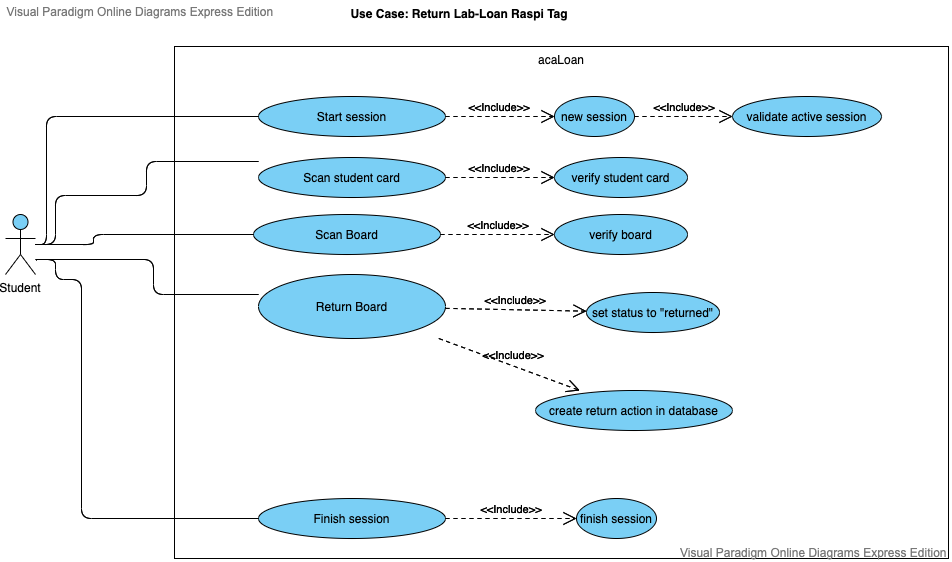
\includegraphics[width=1\textwidth]{gfx/lab_return.png}}
	\caption{UML Anwendungsfall: Rückgabe des Lab-Loan Boards}
	\label{fig:use_lab_return}
\end{figure}

\subsection{Rückgabe des Lab-Loan Boards}
\label{sec:design:use_cases:lab_return}
Das erfolgreichen Szenario als folgenden vorgesehen: nachdem hat ein Studierende mit einem Lab-Loan Board im Raum PSE-Labor angekommen ist, drückt er die Start-Taste am Bildschirm des Display-Client. Dann lässt er seine Studentenkarte am Register-Client über RFID-Leser abzulesen und danach sieht eine Begrüßung des Systems und seinen eigenen Name. Ein Studierende mithilfe des RFID-Lesers liest als nächsten der RFID-Tag des Lab-Loan Board ab, dessen Nummer wird nach dem Ablesen am Bildschirm des Display-Client unter dem Name der Studierende gezeigt. Dann muss die Taste "Return Board" gedrückt werden. Nach der Bestätigung der Rückgabe drückt der Studierende eine Taste "Finish" und somit wird Anwendungsfall erfolgreich beendet. Der oben geschrieben Anwendungsfall ist auf der Abbildung \ref{fig:use_lab_return} zu sehen.

Es sind auch Fehlerzustände für den Anwendungsfall vorgesehen. Es wird die gleiche Fehlerzustände \textit{"Invalid student card"} und \textit{"Status error"} benutzt. Darüber hinaus wird ein Fehlerzustand  \textit{"Return error"} vorgesehen, falls es zum einem Versuch käme, ein Lab-Board zurückzugeben, der nicht von angemeldeten in der Sitzung Studierende ausgeliehen wurde. 

\subsection{Rückgabe des Home-Loan Boards}
\label{sec:design:use_cases:home_return}
Der folgenden Anwendungsfall ist ähnlich zum vorherigen Anwendungsfall \textit{"Rückgabe des Lab-Loan Boards"} aus dem Kapitel \ref{sec:design:use_cases:lab_loan}. Es wird keine erweiterten Beschreibung des Anwendungsfall benötigt, da erfolgreichen Szenario wiederholt sich. Es ist erwartet, dass bei den Home-Loan Boards es häufiger sein kann, dass Board nicht rechtzeitig von einem Studierende zurückgegeben wird. Falls der Rückgabeltermin versäumt ist, wird trotzdem ein Board ohne Fehlermeldung zurückgenommen, da die Rückkehr alle Boards ins Labor hat höher Priorität als die Fehlermeldungen, wegen deren den Studierende überhaupt ablehnen können, Board zurückzugeben. Das gleiche gilt für den Anwendungsfall \textit{"Rückgabe des Home-Loan Boards"}. 

\section{Systemarchitektur}
\label{sec:design:uml}
Die Architektur besteht aus den grundlegenden Beschreibungen (Ansichten),  die zeigen, aus welchen grundlegenden Teilen (Komponenten, Modulen, Layouts usw.) das System besteht und wie diese Beschreibungen zusammenhängen. 

\subsection{Komponentendiagramm}
\label{sec:design:uml:uml_component}
UML-Komponentendiagramme stellen die Beziehungen zwischen einzelnen Systemkomponenten in einer statischen Entwurfssicht dar. Dabei können sowohl logische als auch physische Modellierungsaspekte berücksichtigt werden. Im UML-Kontext sind Komponenten modulare Teile eines Systems, die unabhängig sind und durch äquivalente Komponenten ausgetauscht werden können. Sie sind in sichgeschlossen und kapseln beliebig komplexe Strukturen. Kontakt zu anderen Komponenten nehmen die gekapselten Elemente ausschließlich über Schnittstellen auf\cite{website:20}. Die Komponentendiagramm eines zu entwickelten System ist auf der Abbildung \ref{fig:components} gezeichnet. Die Komponenten werden miteinander über HTTP-Protokoll kommunizieren. Es wird mithilfe API-Endpunkt geschehen, an dem eine Verbindung mit den drei Bestandteilen der Softwareprogramm herstellt wird. An den API-Endpunkt werden Informationsanforderungen von einer Webanwendung einem Webserver geschickt und die Antwort empfangen.
\begin{figure}
	\centering
	\fbox{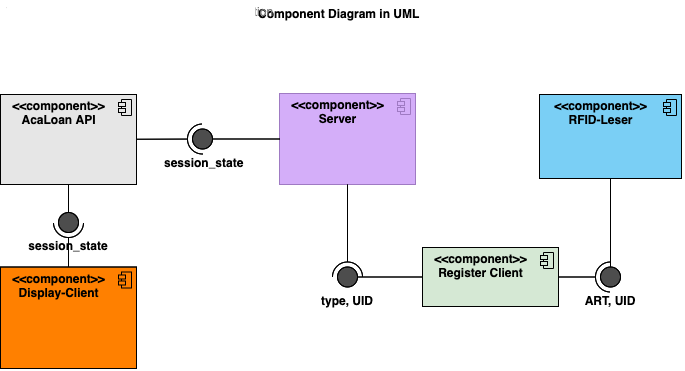
\includegraphics[width=1\textwidth]{gfx/component.png}}
	\caption{UML Komponentendiagramm}
	\label{fig:components}
\end{figure}
Obwohl das Thema der Bachelorarbeit "Entwicklung eine Datenbank-Applikation" lautet, besteht sie nicht nur aus einziger Komponente wie eine Datenbank zur Ausleihverwaltung. Die Aufgabestellung lässt sich die folgenden Struktur definieren, indem drei verteilte Teilen zu entwickeln ist.
\begin{itemize}
	\item Erstens wird an einem uComputer ein sogenannten Register-Client realisiert. Dafür ein RFID-Leser an uComputer angeschlossen wird. Register-Client ist neben dem Eingangstür eines kleinen Lagerraums des PSE-Labors zu platzieren ist, wo Raspi-Boards aufbewahrt werden. Es ist geplant, dass Studierende einen Board selbst aus dem Fach nehmen könnte und dann mit Hilfe des Register-Clients den genommenen Board auf sich oder seine Gruppe registrieren lassen. Der Register-Client hat selbst keinen Zugriff zur Datenbank und sollte nur die abgelesene Daten von der Smartcard der Studierende zur Server schicken. 
	\item Zweitens ist ein Display-Client zu entwickeln, der den Studierenden es zulässt, die Begrüßung des System und eine Beschreibung die für Ausleihe notwendigen Schritten zu sehen. Es sollte in einem Browser-Fenster die aktuelle Server-Kommunikation und Auskunft angezeigt wird, ob die Ausleihe gelang oder ein Fehler aufgetreten war. Ein Android/iOS-Tablett ist eine gute Wahl für die technische Realisierung, da es die Kommunikation zwischen den Mensch und das System leicht und ohne erweiterte Hinweise zulässt. 
	\item Drittens ist ein Web-Server für die Datenbank-Applikation schließlich zu implementieren. Er umfasst alle Datensätze über die vorhandenen im Labor Raspi-Boards, registrierten zum Kurs Studierenden und die abgewickelten Leihvorgänge.  Web-Server wird mit einem Web-Framework Django erstellt. Django verfügt nun über die Funktionalität und Datenbasis, um die dafür erforderlichen Aktionen durchzuführen. Als Web-Framework bietet Django eine Reihe von Komponenten und Funktionen (Benutzerauthentifizierung, Hochladen von Dateien, Umgang mit Daten usw.), die bei jeder Webanwendungen benötigt werden. Mit einem Web-Framework muss ein Entwickler keine Zeit damit verschwenden, denselben Code von Grund auf neu jedes Mal zu schreiben.
	\item Zwischen Server und Klient wird RESTful Kommunikation, die eine Implementierung eines Webdienstes unter Verwendung von HTTP- und REST-Prinzipien ist.
\end{itemize}

Wie erfolgt nun die Abwicklung des eigentlichen Leihvorgangs von der Ausleihe bis zur Rückgabe eines Boards?  Zuerst wird eine Studentenkarte am Register-Client ablesen und nachdem sollte einen Name und die Anzahl schon ausgeliehenen Boards am Display-Client angezeigt werden. Falls der Studierende zum Kurs zugelassen ist, darf dann ein gewünschten Board am Register-Client abgelesen werden. Es ist möglich, dass zu den schon ausgeliehenen Lab-Board noch zusätzlich einen Home-Board nach Hause mitgenommen wird. Das abgelesene Board ist entweder auszuleihen oder zurückzugeben. Sämtliche im Verleih befindlichen Geräte werden von den Mitarbeitern des Labors regelmäßig nach jeder Übung vor dem nächsten Ausleihevorgang auf Funktionsfähigkeit geprüft. Es kann sein, dass einem Studierenden die Home-Loan-Absicht eines Boards (12-16) verweigert wird, da in der Vergangenheit schon einmal vom Studierende ein Board in einem inakzeptabel Zustand zurückgeben war und die Ursachen mit den Mitarbeiter des Labor nicht geklären hat. Falls der Studierende, dem Home-Loan verboten wurde, ein Board auszuleihen versucht, wird eine Fehlermeldung auf dem Bildschirm gezeigt und der Leihvorgang mit dem Fehlerzustand terminiert.  

\subsection{Klassendiagramm}
\label{sec:design:uml:class}
Für das Systemarchitektur wird das UML-Klassendiagramm entwickelt, das einen Überblick über ein Softwaresystem bietet, indem Klassen, Attribute, Operationen und deren Beziehungen angezeigt werden\cite{website:19}. In der Entwurfsphase wird es festgelegt, welche Klassen das System benötigt wird. Die festgestellte Klassen werden weiter nicht wie üblichen Python-Klassen implementieren, jedoch wie eine Django Modelle direkt zum Erzeugen der Datenbank verwendet. Das Klassendiagramm erklärt, was sind die Komponenten des Systems und wo sollen wir die Einkapselungsbarrieren platzieren. Welche Entscheidungen sind innerhalb von Komponenten zu verbergen, damit sie geändert werden können, ohne den Rest des Systems zu beeinträchtigen. Die geplante Klassen sind auf der Abbildung \ref{fig:class} gezeichnet.
\begin{figure}
	\centering
	\fbox{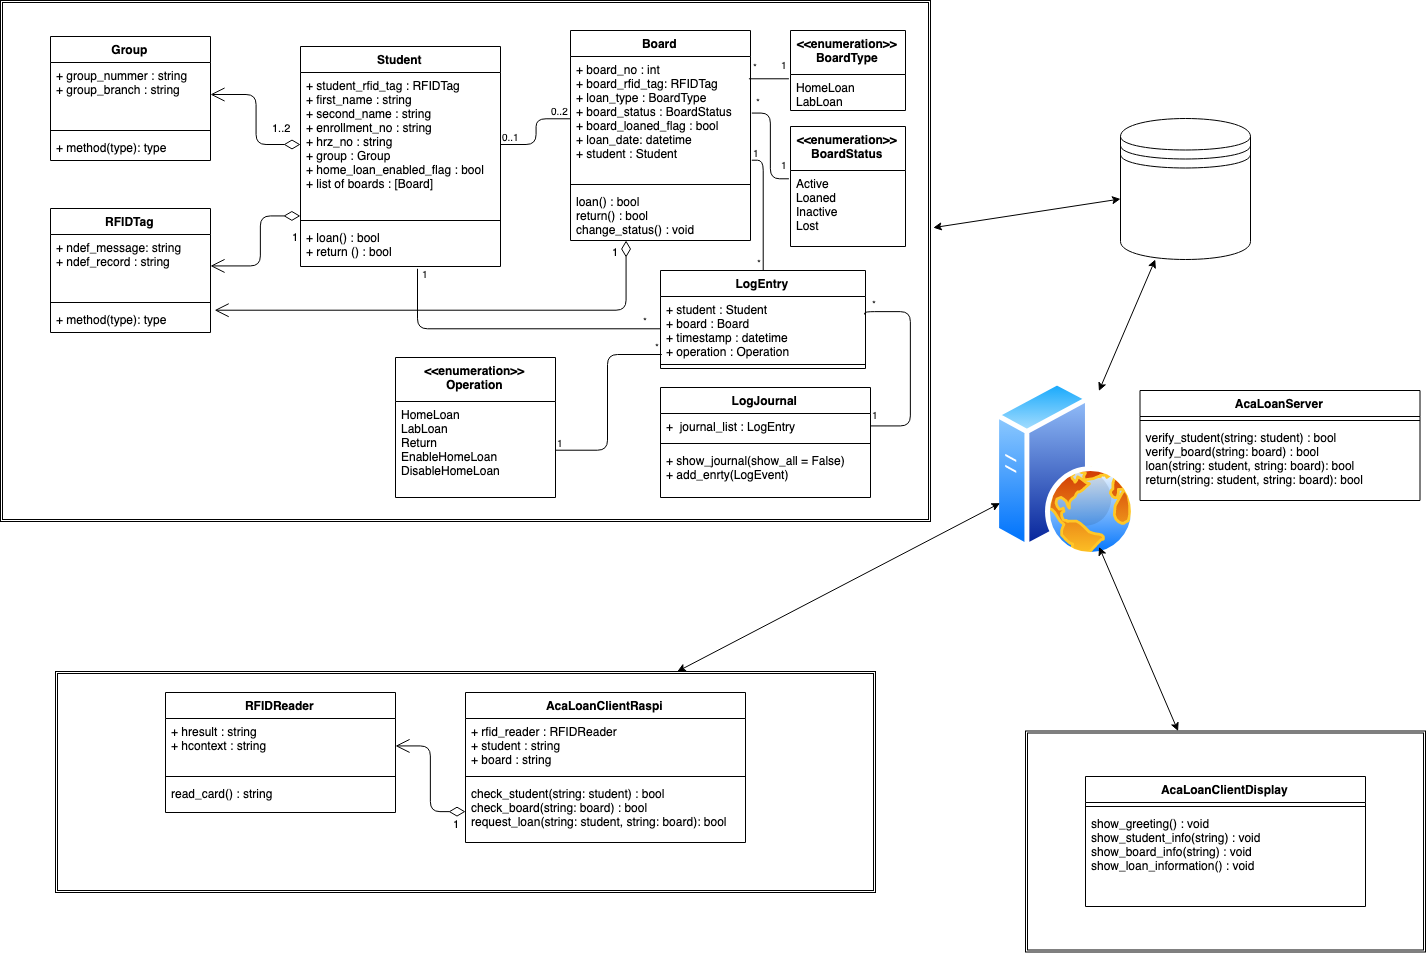
\includegraphics[width=1\textwidth]{gfx/Class_Diagram.png}}
	\caption{UML Klassendiagramm}
	\label{fig:class}
\end{figure}

\section{Endliche Zustandsmaschine}
\label{sec:design:fsm}
Eine Endliche Zustandsmaschine (oder einfach FSM - Finite-State-Maschine) wird für den Sitzungszustand verwendet, da immer nur ein Zustand aktiv sein kann. Um eine Aktion auszuführen, muss die Maschine daher ihren Status ändern. Zustandsmaschine für die Realisierung der Abschlussarbeit wird verwendet, um den Ausführungsfluss zu organisieren und darzustellen. Eine Sitzung wird mit dem Startzustand  \textit{"session started"} angefangen, mit der erfolgreichen Transition \textit{"student card inserted"} in den Zustand \textit{"valid student card"} gewechselt. In diesem Zustand wird den Studierende seinen Name und Vorname auf Bildschirm der Display-Client angezeigt. Es macht keinen Sinn alle Zustände schriftlich zu beschreiben, da diese auf der Abbildung \ref{fig:fsm} abgebildet sind. Die Implementierung der endlichen Zustandsmaschine erfolgt mit django-fsm, die eine einfache deklarative Statusverwaltung für Django-Modelle hinzufügt.

\begin{figure}
	\centering
	\fbox{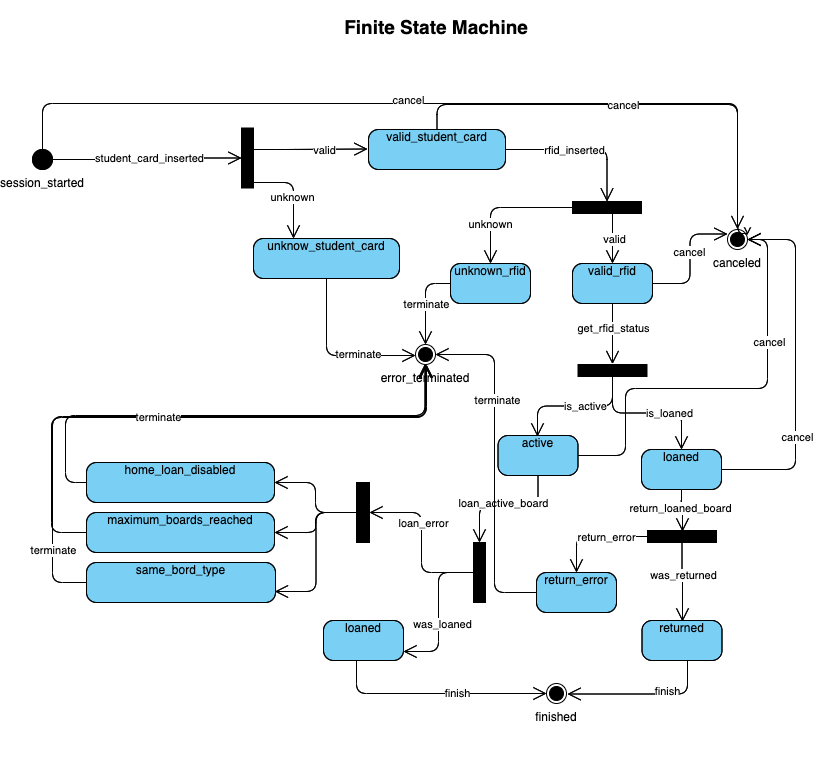
\includegraphics[width=1\textwidth]{gfx/fsm.png}}
	\caption{Endliche Zustandsmaschine}
	\label{fig:fsm}
\end{figure}